\documentclass[ignorenonframetext,]{beamer}
\setbeamertemplate{caption}[numbered]
\setbeamertemplate{caption label separator}{: }
\setbeamercolor{caption name}{fg=normal text.fg}
\beamertemplatenavigationsymbolsempty
\usepackage{lmodern}
\usepackage{amssymb,amsmath}
\usepackage{ifxetex,ifluatex}
\usepackage{fixltx2e} % provides \textsubscript
\ifnum 0\ifxetex 1\fi\ifluatex 1\fi=0 % if pdftex
  \usepackage[T1]{fontenc}
  \usepackage[utf8]{inputenc}
\else % if luatex or xelatex
  \ifxetex
    \usepackage{mathspec}
  \else
    \usepackage{fontspec}
  \fi
  \defaultfontfeatures{Ligatures=TeX,Scale=MatchLowercase}
\fi
% use upquote if available, for straight quotes in verbatim environments
\IfFileExists{upquote.sty}{\usepackage{upquote}}{}
% use microtype if available
\IfFileExists{microtype.sty}{%
\usepackage{microtype}
\UseMicrotypeSet[protrusion]{basicmath} % disable protrusion for tt fonts
}{}
\newif\ifbibliography
\hypersetup{
            pdftitle={Class 8: Bayesian Linear and generalised linear models (GLMs)},
            pdfauthor={Andrew Parnell},
            pdfborder={0 0 0},
            breaklinks=true}
\urlstyle{same}  % don't use monospace font for urls
\usepackage{color}
\usepackage{fancyvrb}
\newcommand{\VerbBar}{|}
\newcommand{\VERB}{\Verb[commandchars=\\\{\}]}
\DefineVerbatimEnvironment{Highlighting}{Verbatim}{commandchars=\\\{\}}
% Add ',fontsize=\small' for more characters per line
\usepackage{framed}
\definecolor{shadecolor}{RGB}{248,248,248}
\newenvironment{Shaded}{\begin{snugshade}}{\end{snugshade}}
\newcommand{\KeywordTok}[1]{\textcolor[rgb]{0.13,0.29,0.53}{\textbf{#1}}}
\newcommand{\DataTypeTok}[1]{\textcolor[rgb]{0.13,0.29,0.53}{#1}}
\newcommand{\DecValTok}[1]{\textcolor[rgb]{0.00,0.00,0.81}{#1}}
\newcommand{\BaseNTok}[1]{\textcolor[rgb]{0.00,0.00,0.81}{#1}}
\newcommand{\FloatTok}[1]{\textcolor[rgb]{0.00,0.00,0.81}{#1}}
\newcommand{\ConstantTok}[1]{\textcolor[rgb]{0.00,0.00,0.00}{#1}}
\newcommand{\CharTok}[1]{\textcolor[rgb]{0.31,0.60,0.02}{#1}}
\newcommand{\SpecialCharTok}[1]{\textcolor[rgb]{0.00,0.00,0.00}{#1}}
\newcommand{\StringTok}[1]{\textcolor[rgb]{0.31,0.60,0.02}{#1}}
\newcommand{\VerbatimStringTok}[1]{\textcolor[rgb]{0.31,0.60,0.02}{#1}}
\newcommand{\SpecialStringTok}[1]{\textcolor[rgb]{0.31,0.60,0.02}{#1}}
\newcommand{\ImportTok}[1]{#1}
\newcommand{\CommentTok}[1]{\textcolor[rgb]{0.56,0.35,0.01}{\textit{#1}}}
\newcommand{\DocumentationTok}[1]{\textcolor[rgb]{0.56,0.35,0.01}{\textbf{\textit{#1}}}}
\newcommand{\AnnotationTok}[1]{\textcolor[rgb]{0.56,0.35,0.01}{\textbf{\textit{#1}}}}
\newcommand{\CommentVarTok}[1]{\textcolor[rgb]{0.56,0.35,0.01}{\textbf{\textit{#1}}}}
\newcommand{\OtherTok}[1]{\textcolor[rgb]{0.56,0.35,0.01}{#1}}
\newcommand{\FunctionTok}[1]{\textcolor[rgb]{0.00,0.00,0.00}{#1}}
\newcommand{\VariableTok}[1]{\textcolor[rgb]{0.00,0.00,0.00}{#1}}
\newcommand{\ControlFlowTok}[1]{\textcolor[rgb]{0.13,0.29,0.53}{\textbf{#1}}}
\newcommand{\OperatorTok}[1]{\textcolor[rgb]{0.81,0.36,0.00}{\textbf{#1}}}
\newcommand{\BuiltInTok}[1]{#1}
\newcommand{\ExtensionTok}[1]{#1}
\newcommand{\PreprocessorTok}[1]{\textcolor[rgb]{0.56,0.35,0.01}{\textit{#1}}}
\newcommand{\AttributeTok}[1]{\textcolor[rgb]{0.77,0.63,0.00}{#1}}
\newcommand{\RegionMarkerTok}[1]{#1}
\newcommand{\InformationTok}[1]{\textcolor[rgb]{0.56,0.35,0.01}{\textbf{\textit{#1}}}}
\newcommand{\WarningTok}[1]{\textcolor[rgb]{0.56,0.35,0.01}{\textbf{\textit{#1}}}}
\newcommand{\AlertTok}[1]{\textcolor[rgb]{0.94,0.16,0.16}{#1}}
\newcommand{\ErrorTok}[1]{\textcolor[rgb]{0.64,0.00,0.00}{\textbf{#1}}}
\newcommand{\NormalTok}[1]{#1}
\usepackage{graphicx,grffile}
\makeatletter
\def\maxwidth{\ifdim\Gin@nat@width>\linewidth\linewidth\else\Gin@nat@width\fi}
\def\maxheight{\ifdim\Gin@nat@height>\textheight0.8\textheight\else\Gin@nat@height\fi}
\makeatother
% Scale images if necessary, so that they will not overflow the page
% margins by default, and it is still possible to overwrite the defaults
% using explicit options in \includegraphics[width, height, ...]{}
\setkeys{Gin}{width=\maxwidth,height=\maxheight,keepaspectratio}

% Prevent slide breaks in the middle of a paragraph:
\widowpenalties 1 10000
\raggedbottom

\AtBeginPart{
  \let\insertpartnumber\relax
  \let\partname\relax
  \frame{\partpage}
}
\AtBeginSection{
  \ifbibliography
  \else
    \let\insertsectionnumber\relax
    \let\sectionname\relax
    \frame{\sectionpage}
  \fi
}
\AtBeginSubsection{
  \let\insertsubsectionnumber\relax
  \let\subsectionname\relax
  \frame{\subsectionpage}
}

\setlength{\parindent}{0pt}
\setlength{\parskip}{6pt plus 2pt minus 1pt}
\setlength{\emergencystretch}{3em}  % prevent overfull lines
\providecommand{\tightlist}{%
  \setlength{\itemsep}{0pt}\setlength{\parskip}{0pt}}
\setcounter{secnumdepth}{0}
\usepackage{graphicx}
\usepackage{amsmath,amsfonts,amssymb,amsthm,amscd, mathrsfs}
\setbeamertemplate{navigation symbols}{} %%removes bottom line
\setbeamertemplate{footline}[frame number]

\title{Class 8: Bayesian Linear and generalised linear models (GLMs)}
\author{Andrew Parnell\newline \texttt{andrew.parnell@mu.ie}
\newline \vspace{1cm} \newline 
\includegraphics[width=5cm]{MU_logo.jpg}}
\date{}

\begin{document}
\frame{\titlepage}

\begin{frame}[fragile]{Learning outcomes}

\begin{itemize}
\tightlist
\item
  Understand the basic formulation of a GLM in a Bayesian context
\item
  Understand the code for a GLM in \texttt{rstanarm}
\item
  Be able to pick a link function for a given data set
\item
  Know how to check model assumptions for a GLM
\end{itemize}

\end{frame}

\begin{frame}[fragile]{Aside: thinking about the data generating process
for a standard LM}

If we believe that a linear model is appropriate for our data, there are
several ways we could generate data from the model. Here is one way:

\begin{Shaded}
\begin{Highlighting}[]
\NormalTok{N =}\StringTok{ }\DecValTok{10}
\NormalTok{x =}\StringTok{ }\DecValTok{1}\OperatorTok{:}\NormalTok{N}
\NormalTok{y =}\StringTok{ }\KeywordTok{rnorm}\NormalTok{(N, }\DataTypeTok{mean =} \OperatorTok{-}\DecValTok{2} \OperatorTok{+}\StringTok{ }\FloatTok{0.4} \OperatorTok{*}\StringTok{ }\NormalTok{x, }\DataTypeTok{sd =} \DecValTok{1}\NormalTok{)}
\end{Highlighting}
\end{Shaded}

Here is another:

\begin{Shaded}
\begin{Highlighting}[]
\NormalTok{eps =}\StringTok{ }\KeywordTok{rnorm}\NormalTok{(N, }\DataTypeTok{mean =} \DecValTok{0}\NormalTok{, }\DataTypeTok{sd =} \DecValTok{1}\NormalTok{)}
\NormalTok{y =}\StringTok{ }\OperatorTok{-}\DecValTok{2} \OperatorTok{+}\StringTok{ }\FloatTok{0.4} \OperatorTok{*}\StringTok{ }\NormalTok{x }\OperatorTok{+}\StringTok{ }\NormalTok{eps}
\end{Highlighting}
\end{Shaded}

\end{frame}

\begin{frame}[fragile]{The data generating process for a logistic
regression}

\scriptsize
- What if the response variable was binary? Clearly the previous code
will not produce binary values - Instead we could simulate from the
binomial distribution:

\begin{Shaded}
\begin{Highlighting}[]
\NormalTok{y =}\StringTok{ }\KeywordTok{rbinom}\NormalTok{(N, }\DataTypeTok{size =} \DecValTok{1}\NormalTok{, }\DataTypeTok{prob =} \OperatorTok{-}\DecValTok{2} \OperatorTok{+}\StringTok{ }\FloatTok{0.4} \OperatorTok{*}\StringTok{ }\NormalTok{x)}
\end{Highlighting}
\end{Shaded}

\ldots{} but this will produce \texttt{NA}s as the \texttt{prob}
argument needs to be between 0 and 1. We need to transform the values
involving the covariate

\begin{itemize}
\tightlist
\item
  A popular way is to use the inverse logit function. Look!
\end{itemize}

\begin{Shaded}
\begin{Highlighting}[]
\OperatorTok{-}\DecValTok{2} \OperatorTok{+}\StringTok{ }\FloatTok{0.4} \OperatorTok{*}\StringTok{ }\NormalTok{x}
\end{Highlighting}
\end{Shaded}

\begin{verbatim}
##  [1] -1.6 -1.2 -0.8 -0.4  0.0  0.4  0.8  1.2  1.6  2.0
\end{verbatim}

\begin{Shaded}
\begin{Highlighting}[]
\KeywordTok{exp}\NormalTok{(}\OperatorTok{-}\DecValTok{2} \OperatorTok{+}\StringTok{ }\FloatTok{0.4} \OperatorTok{*}\StringTok{ }\NormalTok{x)}\OperatorTok{/}\NormalTok{(}\DecValTok{1} \OperatorTok{+}\StringTok{ }\KeywordTok{exp}\NormalTok{(}\OperatorTok{-}\DecValTok{2} \OperatorTok{+}\StringTok{ }\FloatTok{0.4} \OperatorTok{*}\StringTok{ }\NormalTok{x))}
\end{Highlighting}
\end{Shaded}

\begin{verbatim}
##  [1] 0.1679816 0.2314752 0.3100255 0.4013123 0.5000000 0.5986877 0.6899745
##  [8] 0.7685248 0.8320184 0.8807971
\end{verbatim}

\begin{itemize}
\tightlist
\item
  In fact you can take any number \(a\) from \(-\infty\) to \(\infty\)
  and create \(\exp(a)/(1+\exp(a))\) and it will always lie between 0
  and 1
\end{itemize}

\end{frame}

\begin{frame}[fragile]{Generating binomial data}

\begin{itemize}
\tightlist
\item
  Thus a way to generate binary data which allows for covariates is:
\end{itemize}

\begin{Shaded}
\begin{Highlighting}[]
\KeywordTok{library}\NormalTok{(boot)}
\NormalTok{p =}\StringTok{ }\KeywordTok{inv.logit}\NormalTok{(}\OperatorTok{-}\DecValTok{2} \OperatorTok{+}\StringTok{ }\FloatTok{0.4} \OperatorTok{*}\StringTok{ }\NormalTok{x)}
\NormalTok{y =}\StringTok{ }\KeywordTok{rbinom}\NormalTok{(N, }\DataTypeTok{size =} \DecValTok{1}\NormalTok{, }\DataTypeTok{prob =}\NormalTok{ p)}
\NormalTok{y}
\end{Highlighting}
\end{Shaded}

\begin{verbatim}
##  [1] 0 1 1 1 0 0 1 0 0 1
\end{verbatim}

\begin{itemize}
\tightlist
\item
  The logit function itself is \(\log \left( \frac{p}{1-p} \right)\) and
  will turn the probabilities form the range (0,1) to the range
  \((-\infty,\infty)\)
\item
  Using this type of model is known as \emph{logistic-Binomial}
  regression and the logit is known as the \emph{link function}
\end{itemize}

\end{frame}

\begin{frame}[fragile]{Generating other types of data}

\begin{itemize}
\tightlist
\item
  Once we have discovered link functions, we can use them to generate
  other types of data, e.g.~Poisson data via the log link:
\end{itemize}

\begin{Shaded}
\begin{Highlighting}[]
\NormalTok{lambda =}\StringTok{ }\KeywordTok{exp}\NormalTok{(}\OperatorTok{-}\DecValTok{2} \OperatorTok{+}\StringTok{ }\FloatTok{0.4} \OperatorTok{*}\StringTok{ }\NormalTok{x)}
\NormalTok{y =}\StringTok{ }\KeywordTok{rpois}\NormalTok{(N, lambda)}
\NormalTok{y}
\end{Highlighting}
\end{Shaded}

\begin{verbatim}
##  [1] 0 0 1 1 0 2 2 3 8 2
\end{verbatim}

\begin{itemize}
\tightlist
\item
  The rate (\(\lambda\)) of the Poisson distribution has to be positive,
  so taking the log of it changes its range to \((-\infty,\infty)\) as
  before. The inverse-link (\(\exp\)) turns the unrestricted ranges into
  something that must be positive
\end{itemize}

\end{frame}

\begin{frame}{From LM to GLM}

\begin{itemize}
\item
  In general, a \emph{generalised linear model} (GLM) can be written out
  as: \[y \sim Distribution(f(\theta, x))\] where \(Distribution\) is
  some probability distribution, \(\theta\) are some parameters, and
  \(f\) is a link function that transforms the parameters into a range
  so that we can incorporate \(x\) in an unrestricted way
\item
  The above allows us to simulate from the model, given some parameters
  \(\theta\) and some covariates \(x\) we can use the probability
  distribution to get simulated data
\item
  It also allows us to calculate the \emph{likelihood} as we can get a
  score for how likely it is to see the data we have observed given some
  values of the parameters
\end{itemize}

\end{frame}

\begin{frame}[fragile]{Multiple covariates}

\begin{itemize}
\tightlist
\item
  We can extend LMs and GLMs to have multiple covariates if we want,
  e.g.
\end{itemize}

\begin{Shaded}
\begin{Highlighting}[]
\NormalTok{y =}\StringTok{ }\KeywordTok{rnorm}\NormalTok{(N, }\DataTypeTok{mean =} \OperatorTok{-}\DecValTok{2} \OperatorTok{+}\StringTok{ }\FloatTok{0.4} \OperatorTok{*}\StringTok{ }\NormalTok{x1 }\OperatorTok{-}\StringTok{ }\FloatTok{0.3} \OperatorTok{*}\StringTok{ }\NormalTok{x2, }\DataTypeTok{sd =} \DecValTok{1}\NormalTok{)}
\NormalTok{p =}\StringTok{ }\KeywordTok{inv.logit}\NormalTok{(}\OperatorTok{-}\DecValTok{2} \OperatorTok{+}\StringTok{ }\FloatTok{0.4} \OperatorTok{*}\StringTok{ }\NormalTok{x1 }\OperatorTok{-}\StringTok{ }\FloatTok{0.3} \OperatorTok{*}\StringTok{ }\NormalTok{x2)}
\NormalTok{y =}\StringTok{ }\KeywordTok{rbinom}\NormalTok{(N, }\DataTypeTok{size =} \DecValTok{1}\NormalTok{, }\DataTypeTok{prob =}\NormalTok{ p)}
\end{Highlighting}
\end{Shaded}

\begin{itemize}
\tightlist
\item
  Alternatively we can incorporate multiplicative interactions\ldots{}
\end{itemize}

\begin{Shaded}
\begin{Highlighting}[]
\NormalTok{y =}\StringTok{ }\KeywordTok{rnorm}\NormalTok{(N, }\DataTypeTok{mean =} \OperatorTok{-}\DecValTok{2} \OperatorTok{+}\StringTok{ }\FloatTok{0.4} \OperatorTok{*}\StringTok{ }\NormalTok{x1 }\OperatorTok{-}\StringTok{ }\FloatTok{0.3} \OperatorTok{*}\StringTok{ }\NormalTok{x2 }\OperatorTok{+}\StringTok{ }
\StringTok{            }\FloatTok{0.05} \OperatorTok{*}\StringTok{ }\NormalTok{x1 }\OperatorTok{*}\StringTok{ }\NormalTok{x2, }\DataTypeTok{sd =} \DecValTok{1}\NormalTok{)}
\end{Highlighting}
\end{Shaded}

\begin{itemize}
\tightlist
\item
  \ldots{} or non-linear effects
\end{itemize}

\begin{Shaded}
\begin{Highlighting}[]
\NormalTok{p =}\StringTok{ }\KeywordTok{inv.logit}\NormalTok{(}\OperatorTok{-}\DecValTok{2} \OperatorTok{+}\StringTok{ }\FloatTok{0.4} \OperatorTok{*}\StringTok{ }\NormalTok{x1 }\OperatorTok{-}\StringTok{ }\FloatTok{0.3} \OperatorTok{*}\StringTok{ }\NormalTok{x2 }\OperatorTok{-}\StringTok{ }\FloatTok{0.02} \OperatorTok{*}\StringTok{ }\NormalTok{x1}\OperatorTok{^}\DecValTok{2}\NormalTok{)}
\NormalTok{y =}\StringTok{ }\KeywordTok{rbinom}\NormalTok{(N, }\DataTypeTok{size =} \DecValTok{1}\NormalTok{, }\DataTypeTok{prob =}\NormalTok{ p)}
\end{Highlighting}
\end{Shaded}

\end{frame}

\begin{frame}{Directed Acyclic Graphs}

\begin{itemize}
\tightlist
\item
  Once we have decided on a model, it is often a good idea to draw a
  picture of it to make it clear how it works
\item
  In Bayesian statistics, this is commonly done using a Directed Acyclic
  Graph or DAG which tells us how to simulate from the model. Circles
  indicate parameters, squares data, and the dotted lines indicate loops
\item
  Here is a DAG for the logistic regression model with two covariates:
\end{itemize}

\begin{center}
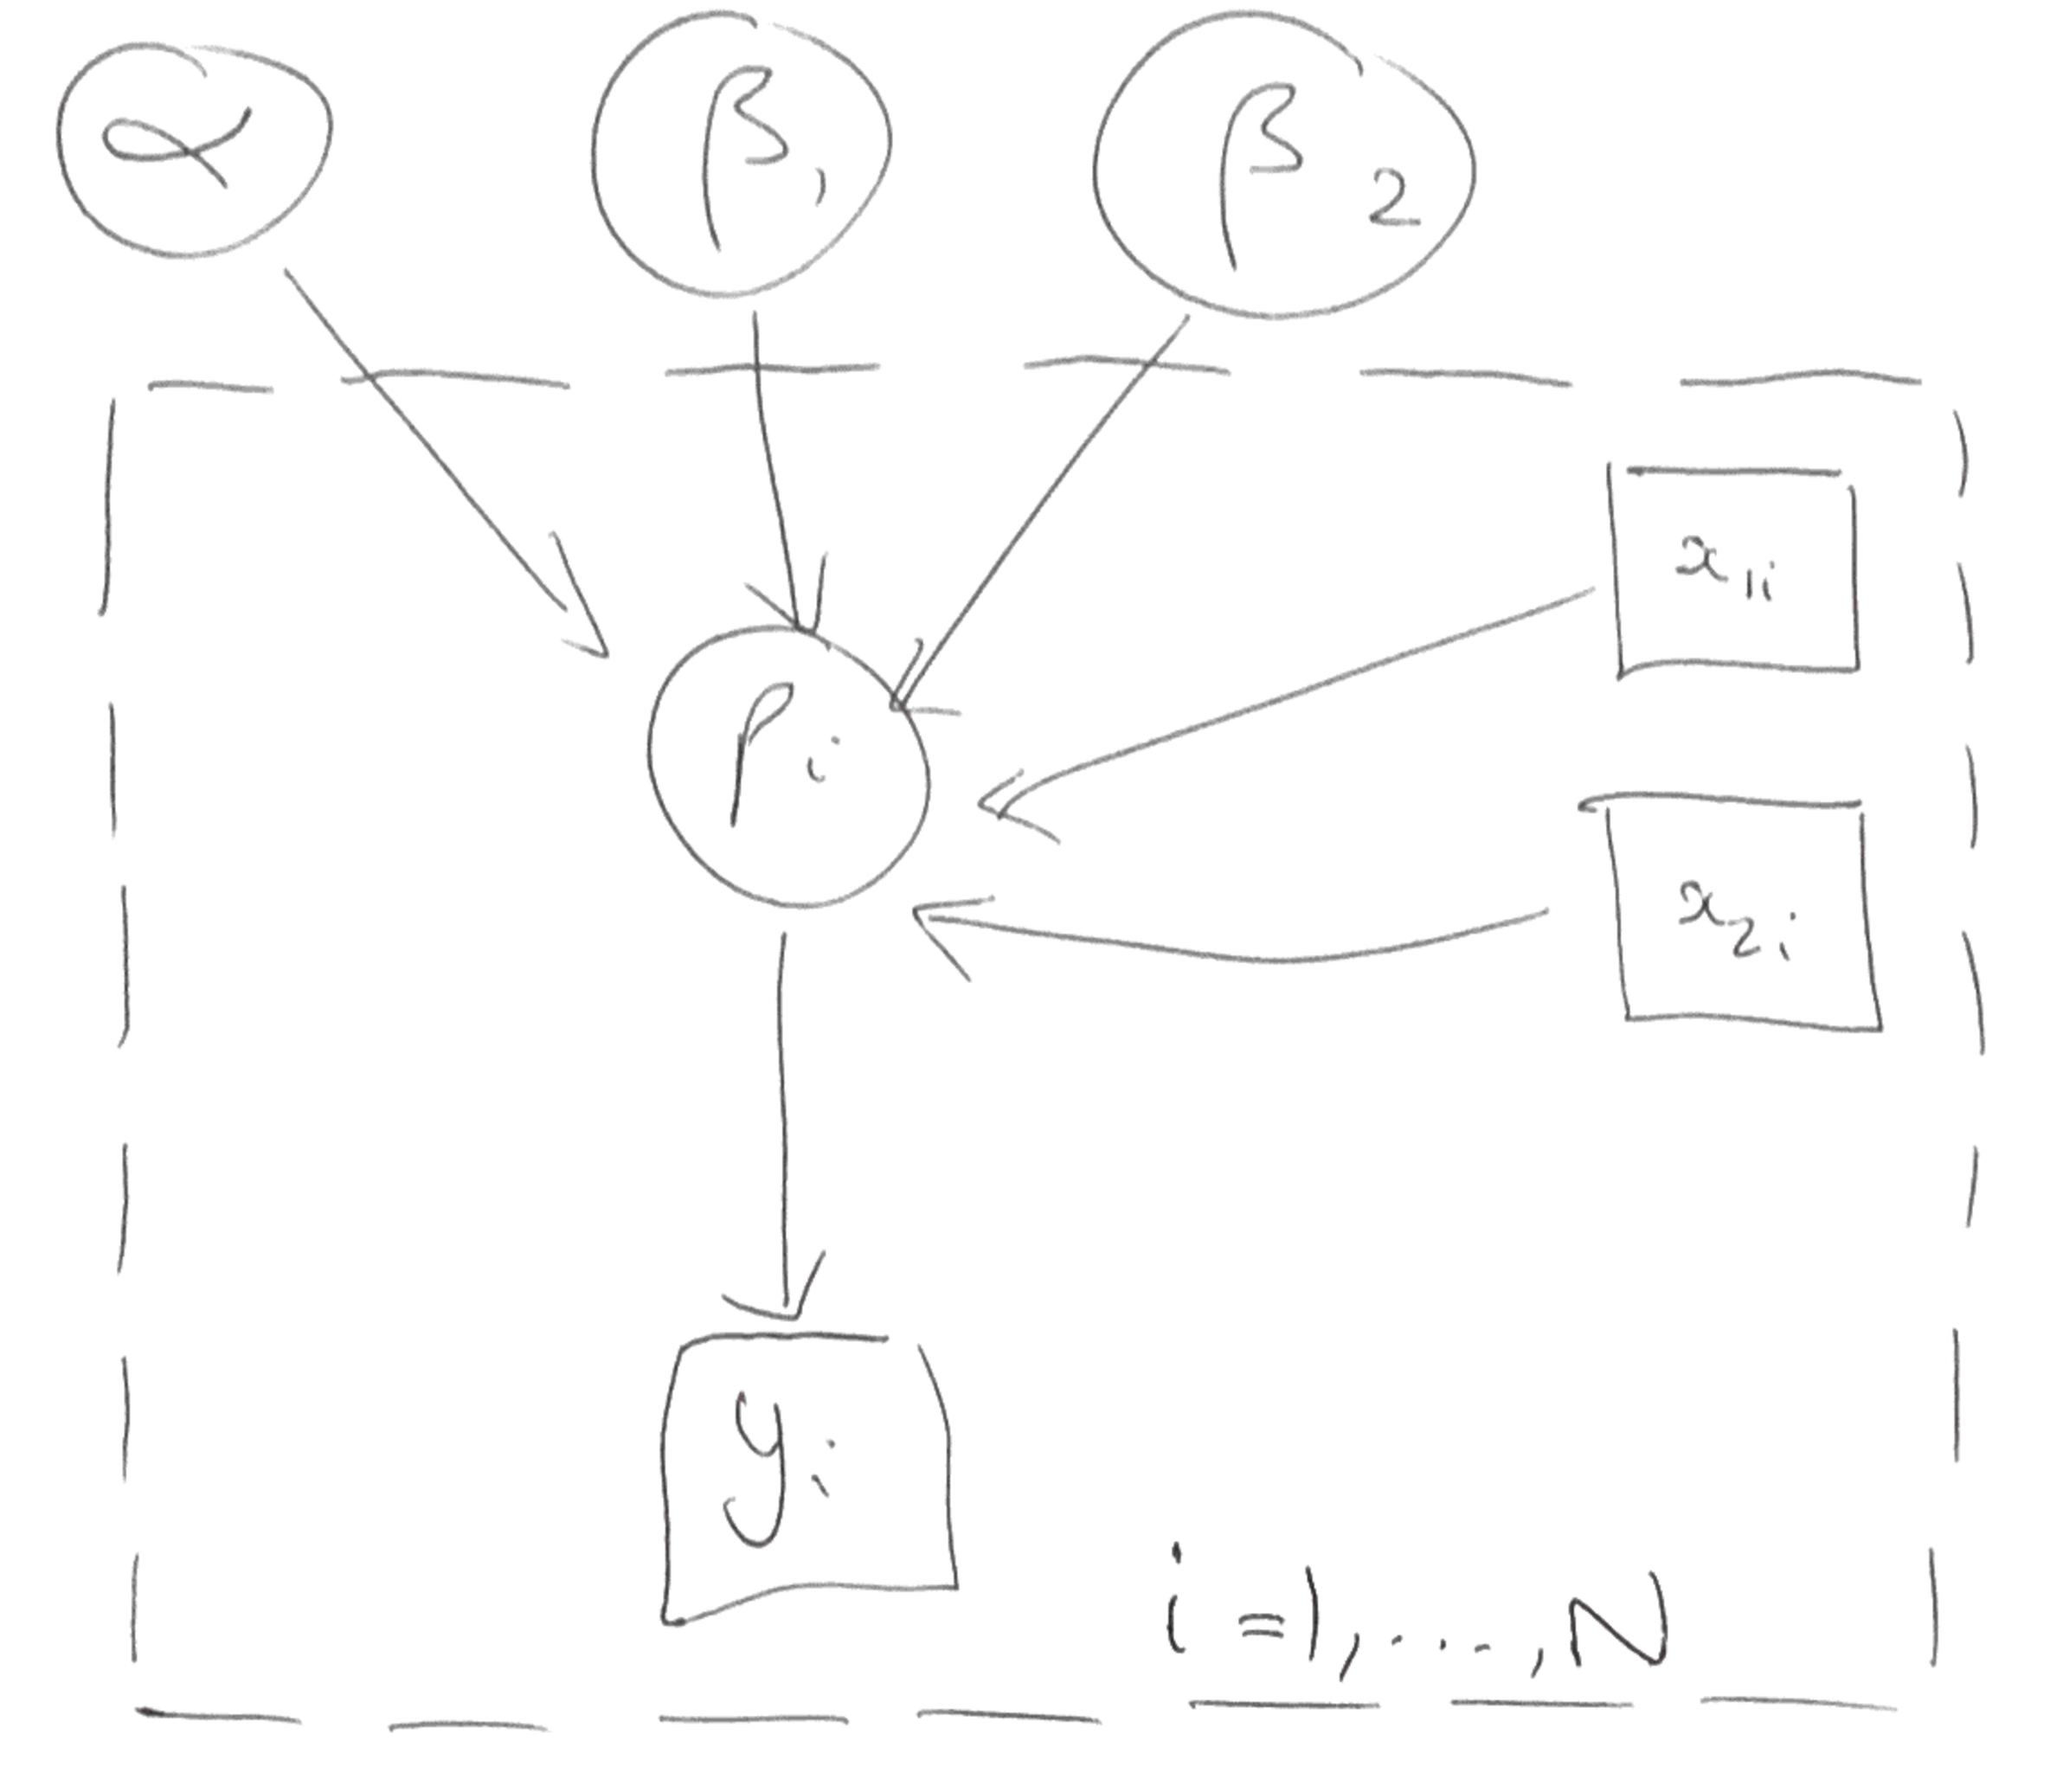
\includegraphics[width=4cm]{DAG.pdf}
\end{center}

\end{frame}

\begin{frame}[fragile]{Example: earnings data}

\begin{itemize}
\tightlist
\item
  Going back to the earnings data, suppose we want to fit a model to
  predict log earnings based on sex and whether respondent is white
  (\texttt{eth==3}) or not
\item
  The model is:
  \[\log(\mbox{earnings}) \sim N(\alpha + \beta_1 \mbox{height} + \beta_2 \mbox{white}, \sigma^2)\]
\item
  We want to get the posterior distribution of
  \(\alpha, \beta_1, \beta_2\) and \(\sigma\) given the data
\item
  What prior distributions could we set on these parameters?
\end{itemize}

\end{frame}

\begin{frame}[fragile]{Fitting linear regression models in rstanarm}

Model code: \tiny

\begin{Shaded}
\begin{Highlighting}[]
\NormalTok{earnings =}\StringTok{ }\KeywordTok{read.csv}\NormalTok{(}\StringTok{'data/earnings.csv'}\NormalTok{)}
\NormalTok{earnings}\OperatorTok{$}\NormalTok{white =}\StringTok{ }\KeywordTok{as.integer}\NormalTok{(earnings}\OperatorTok{$}\NormalTok{eth }\OperatorTok{==}\StringTok{ }\DecValTok{3}\NormalTok{)}
\NormalTok{mod_}\DecValTok{1}\NormalTok{ =}\StringTok{ }\KeywordTok{stan_lm}\NormalTok{(y }\OperatorTok{~}\StringTok{ }\NormalTok{x_centered }\OperatorTok{+}\StringTok{ }\NormalTok{white, }\DataTypeTok{data =}\NormalTok{ earnings,}
                \DataTypeTok{prior =} \KeywordTok{R2}\NormalTok{(}\DataTypeTok{location =} \FloatTok{0.5}\NormalTok{, }\StringTok{'mean'}\NormalTok{))}
\end{Highlighting}
\end{Shaded}

\begin{Shaded}
\begin{Highlighting}[]
\KeywordTok{round}\NormalTok{(}\KeywordTok{as.data.frame}\NormalTok{(}\KeywordTok{summary}\NormalTok{(mod_}\DecValTok{1}\NormalTok{)), }\DecValTok{2}\NormalTok{)}
\end{Highlighting}
\end{Shaded}

\begin{verbatim}
##                   mean mcse   sd     2.5%      25%      50%      75%
## (Intercept)       9.65 0.00 0.07     9.52     9.61     9.65     9.70
## x_centered        0.02 0.00 0.00     0.02     0.02     0.02     0.02
## white             0.10 0.00 0.07    -0.04     0.06     0.10     0.15
## sigma             0.91 0.00 0.02     0.87     0.89     0.91     0.92
## log-fit_ratio     0.00 0.00 0.02    -0.04    -0.01     0.00     0.02
## R2                0.06 0.00 0.01     0.03     0.05     0.06     0.07
## mean_PPD          9.74 0.00 0.04     9.66     9.71     9.74     9.76
## log-posterior -1402.70 0.06 1.82 -1407.13 -1403.66 -1402.36 -1401.36
##                  97.5% n_eff Rhat
## (Intercept)       9.78  1785    1
## x_centered        0.03  2479    1
## white             0.25  1792    1
## sigma             0.95  2620    1
## log-fit_ratio     0.05  2422    1
## R2                0.09  2548    1
## mean_PPD          9.81  4000    1
## log-posterior -1400.21  1038    1
\end{verbatim}

\end{frame}

\begin{frame}[fragile]{Plot the posterior values}

\begin{Shaded}
\begin{Highlighting}[]
\KeywordTok{plot}\NormalTok{(mod_}\DecValTok{1}\NormalTok{)}
\end{Highlighting}
\end{Shaded}

\includegraphics{class_8_bglms_files/figure-beamer/unnamed-chunk-12-1.pdf}

\end{frame}

\begin{frame}[fragile]{Using other priors}

\tiny

\begin{Shaded}
\begin{Highlighting}[]
\NormalTok{mod_}\DecValTok{2}\NormalTok{ =}\StringTok{ }\KeywordTok{stan_lm}\NormalTok{(y }\OperatorTok{~}\StringTok{ }\NormalTok{x_centered }\OperatorTok{+}\StringTok{ }\NormalTok{white, }\DataTypeTok{data =}\NormalTok{ earnings,}
                \DataTypeTok{prior =} \KeywordTok{R2}\NormalTok{(}\DataTypeTok{location =} \FloatTok{0.5}\NormalTok{, }\StringTok{'mean'}\NormalTok{),}
                \DataTypeTok{prior_intercept =} \KeywordTok{normal}\NormalTok{(}\DecValTok{0}\NormalTok{, }\DecValTok{10}\NormalTok{))}
\end{Highlighting}
\end{Shaded}

\begin{Shaded}
\begin{Highlighting}[]
\KeywordTok{round}\NormalTok{(}\KeywordTok{as.data.frame}\NormalTok{(}\KeywordTok{summary}\NormalTok{(mod_}\DecValTok{2}\NormalTok{)), }\DecValTok{2}\NormalTok{)}
\end{Highlighting}
\end{Shaded}

\begin{verbatim}
##                   mean mcse   sd     2.5%      25%      50%      75%
## (Intercept)       9.65 0.00 0.07     9.52     9.61     9.65     9.70
## x_centered        0.02 0.00 0.00     0.02     0.02     0.02     0.02
## white             0.10 0.00 0.07    -0.04     0.05     0.10     0.15
## sigma             0.91 0.00 0.02     0.87     0.89     0.91     0.92
## log-fit_ratio     0.00 0.00 0.02    -0.04    -0.01     0.00     0.02
## R2                0.06 0.00 0.01     0.03     0.05     0.06     0.07
## mean_PPD          9.74 0.00 0.04     9.66     9.71     9.74     9.76
## log-posterior -1404.11 0.06 1.75 -1408.59 -1405.05 -1403.79 -1402.80
##                  97.5% n_eff Rhat
## (Intercept)       9.78  1446    1
## x_centered        0.03  1880    1
## white             0.25  1605    1
## sigma             0.95  2443    1
## log-fit_ratio     0.04  2333    1
## R2                0.09  1974    1
## mean_PPD          9.81  4000    1
## log-posterior -1401.70  1014    1
\end{verbatim}

\end{frame}

\begin{frame}[fragile]{What do the results actually mean?}

\begin{itemize}
\tightlist
\item
  We now have access to the posterior distribution of the parameters:
\end{itemize}

\begin{Shaded}
\begin{Highlighting}[]
\NormalTok{post =}\StringTok{ }\KeywordTok{as.data.frame}\NormalTok{(mod_}\DecValTok{2}\NormalTok{)}
\KeywordTok{head}\NormalTok{(post)}
\end{Highlighting}
\end{Shaded}

\begin{verbatim}
##   (Intercept) x_centered      white     sigma log-fit_ratio         R2
## 1    9.592836 0.02507382 0.21633742 0.9301058  0.0360975405 0.07399261
## 2    9.551875 0.02282112 0.17018098 0.9139646  0.0123258219 0.06231639
## 3    9.588871 0.02163994 0.15578411 0.8900420 -0.0160066247 0.05891715
## 4    9.589588 0.02174304 0.20310271 0.9158380  0.0128601927 0.05947395
## 5    9.599199 0.02180863 0.19532988 0.9138107  0.0106283403 0.05944437
## 6    9.680555 0.01996215 0.04551595 0.9121066  0.0007152551 0.04418558
\end{verbatim}

\end{frame}

\begin{frame}[fragile]{Plots of output}

\begin{Shaded}
\begin{Highlighting}[]
\KeywordTok{library}\NormalTok{(bayesplot)}
\KeywordTok{mcmc_areas}\NormalTok{(post,}
           \DataTypeTok{pars =} \KeywordTok{c}\NormalTok{(}\StringTok{"x_centered"}\NormalTok{, }\StringTok{"white"}\NormalTok{, }\StringTok{"sigma"}\NormalTok{))}
\end{Highlighting}
\end{Shaded}

\includegraphics{class_8_bglms_files/figure-beamer/unnamed-chunk-16-1.pdf}

\end{frame}

\begin{frame}[fragile]{\texttt{rstan} version}

\begin{Shaded}
\begin{Highlighting}[]
\NormalTok{stan_code =}\StringTok{ '}
\StringTok{data \{}
\StringTok{  int<lower=0> N;}
\StringTok{  vector[N] y;}
\StringTok{  vector[N] x1;}
\StringTok{  vector[N] x2;}
\StringTok{\}}
\StringTok{parameters \{}
\StringTok{  real alpha;}
\StringTok{  real beta1;}
\StringTok{  real beta2;}
\StringTok{  real<lower=0> sigma;}
\StringTok{\}}
\StringTok{model \{}
\StringTok{  y ~ normal(alpha + x1 * beta1  + x2 * beta2, sigma);}
\StringTok{\}}
\StringTok{'}
\end{Highlighting}
\end{Shaded}

\end{frame}

\begin{frame}[fragile]{Running the Stan version}

\begin{Shaded}
\begin{Highlighting}[]
\KeywordTok{library}\NormalTok{(rstan)}
\NormalTok{stan_run =}\StringTok{ }\KeywordTok{stan}\NormalTok{(}\DataTypeTok{data =} \KeywordTok{list}\NormalTok{(}\DataTypeTok{N =} \KeywordTok{nrow}\NormalTok{(earnings), }
                            \DataTypeTok{y =}\NormalTok{ earnings}\OperatorTok{$}\NormalTok{y,}
                            \DataTypeTok{x1 =}\NormalTok{ earnings}\OperatorTok{$}\NormalTok{x, }
                            \DataTypeTok{x2 =}\NormalTok{ earnings}\OperatorTok{$}\NormalTok{white),}
                \DataTypeTok{model_code =}\NormalTok{ stan_code)}
\end{Highlighting}
\end{Shaded}

\end{frame}

\begin{frame}[fragile]{Stan output}

\begin{Shaded}
\begin{Highlighting}[]
\KeywordTok{plot}\NormalTok{(stan_run)}
\end{Highlighting}
\end{Shaded}

\includegraphics{class_8_bglms_files/figure-beamer/unnamed-chunk-19-1.pdf}

\end{frame}

\begin{frame}[fragile]{To standardise or not?}

\begin{itemize}
\tightlist
\item
  Most regression models work better if the covariates are standardised
  (subtract the mean and divide by the standard deviation) before you
  run the model
\item
  \texttt{rstan} can struggle with regression models where the data are
  not standardised. \texttt{rstanarm} does a much better job
\item
  The advantage of standardising is that you get more numerically stable
  results (this is true of \texttt{R}'s \texttt{lm} function too), and
  that you can directly compare between the different slopes
\item
  The disadvantage is that the slope values are no longer in the
  original units (e.g.~cm)
\end{itemize}

\end{frame}

\begin{frame}{What is stan doing in the background?}

\begin{itemize}
\item
  Stans run a stochastic algorithm called Hamiltonian Monte Carlo to
  create the samples from the posterior distribution
\item
  This involves:

  \begin{enumerate}
  \def\labelenumi{\arabic{enumi}.}
  \tightlist
  \item
    Guessing at \emph{initial values} of the parameters. Scoring these
    against the likelihood and the prior to see how well they match the
    data
  \item
    Then iterating:

    \begin{enumerate}
    \def\labelenumii{\arabic{enumii}.}
    \tightlist
    \item
      Working out which \emph{directions} to try to generate new good
      parameter values
    \item
      Sampling \emph{new parameter values} which may or may not be
      similar to the previous values
    \item
      Repeating these steps to build up a posterior sample of parameter
      values
    \end{enumerate}
  \end{enumerate}
\item
  What you end up with is a set of parameter values for however many
  iterations you chose.
\end{itemize}

\end{frame}

\begin{frame}[fragile]{How many iterations?}

\begin{itemize}
\item
  Ideally you want a set of posterior parameter samples that are
  independent across iterations and is of sufficient size that you can
  get decent estimates of uncertainty
\item
  There are three key parts of the algorithm that affect how good the
  posterior samples are:

  \begin{enumerate}
  \def\labelenumi{\arabic{enumi}.}
  \tightlist
  \item
    The starting values you chose. If you chose bad starting values, you
    might need to discard the first few thousand iterations. This is
    known as the \emph{burn-in} period
  \item
    The way you choose your new parameter values. If they are too close
    to the previous values the MCMC might move too slowly so you might
    need to \emph{thin} the samples out by taking e.g.~every 5th or 10th
    iteration
  \item
    The total number of iterations you choose. Ideally you would take
    millions but this will make the run time slower
  \end{enumerate}
\end{itemize}

\texttt{rstanarm} and \texttt{rstan} have good default choices for these
but for complex models you often need to intervene

\end{frame}

\begin{frame}[fragile]{Plotting the iterations}

You can plot the iterations for all the parameters with
\texttt{mcmc\_trace}, e.g.

\begin{Shaded}
\begin{Highlighting}[]
\KeywordTok{mcmc_trace}\NormalTok{(post, }\DataTypeTok{pars =} \KeywordTok{c}\NormalTok{(}\StringTok{'white'}\NormalTok{, }\StringTok{'x_centered'}\NormalTok{, }\StringTok{'sigma'}\NormalTok{),}
           \DataTypeTok{facet_args =} \KeywordTok{list}\NormalTok{(}\DataTypeTok{nrow =} \DecValTok{3}\NormalTok{))}
\end{Highlighting}
\end{Shaded}

\includegraphics{class_8_bglms_files/figure-beamer/unnamed-chunk-20-1.pdf}

A good trace plot will show no patterns or runs, and will look like it
has a stationary mean and variance

\end{frame}

\begin{frame}[fragile]{How many chains?}

\begin{itemize}
\tightlist
\item
  Beyond increasing the number of iterations, thinning, and removing a
  burn-in period, Stan automatically runs \emph{multiple chains}
\item
  This means that they start the algorithm from 3 or 4 different sets of
  starting values and see if each \emph{chain} converges to the same
  posterior distribution
\item
  If the MCMC algorithm has converged then each chain should have the
  same mean and variance.
\item
  Stan reports the \texttt{Rhat} value, which is close to 1 when all the
  chains match
\item
  It's about the simplest and quickest way to check convergence. If you
  get \texttt{Rhat} values above 1.1, run your MCMC for more iterations
\end{itemize}

\end{frame}

\begin{frame}[fragile]{What else can I do with the output}

\begin{itemize}
\tightlist
\item
  We could create \emph{credible intervals} (Bayesian confidence
  intervals):
\end{itemize}

\tiny

\begin{Shaded}
\begin{Highlighting}[]
\KeywordTok{mcmc_intervals}\NormalTok{(post)}
\end{Highlighting}
\end{Shaded}

\includegraphics{class_8_bglms_files/figure-beamer/unnamed-chunk-21-1.pdf}

\end{frame}

\begin{frame}[fragile]{Or histograms}

\tiny

\begin{Shaded}
\begin{Highlighting}[]
\KeywordTok{mcmc_hist}\NormalTok{(post)}
\end{Highlighting}
\end{Shaded}

\begin{verbatim}
## `stat_bin()` using `bins = 30`. Pick better value with `binwidth`.
\end{verbatim}

\includegraphics{class_8_bglms_files/figure-beamer/unnamed-chunk-22-1.pdf}

\end{frame}

\begin{frame}{Checking model fit}

\begin{itemize}
\tightlist
\item
  How do we know if this model fits the data well or not?
\item
  One way is to simulate from the posterior distribution of the
  parameters, and subsequently simulate from the likelihood to see if
  the these data match the real data we observed
\item
  This is known as a \emph{posterior predictive check}
\end{itemize}

\end{frame}

\begin{frame}[fragile]{Posterior predictive: the long way}

\begin{itemize}
\tightlist
\item
  The long way of doing this is in R after running the model
\item
  For each value sampled from the posterior, compute:
\end{itemize}

\begin{Shaded}
\begin{Highlighting}[]
\NormalTok{y_sim =}\StringTok{ }\KeywordTok{rnorm}\NormalTok{(}\KeywordTok{nrow}\NormalTok{(earnings), }
\NormalTok{              post}\OperatorTok{$}\StringTok{`}\DataTypeTok{(Intercept)}\StringTok{`}\NormalTok{[}\DecValTok{1}\NormalTok{] }\OperatorTok{+}\StringTok{ }
\StringTok{                }\NormalTok{post}\OperatorTok{$}\NormalTok{x_centered[}\DecValTok{1}\NormalTok{] }\OperatorTok{*}\StringTok{ }\NormalTok{earnings}\OperatorTok{$}\NormalTok{x_centered }\OperatorTok{+}\StringTok{ }
\StringTok{                }\NormalTok{post}\OperatorTok{$}\NormalTok{white[}\DecValTok{1}\NormalTok{] }\OperatorTok{*}\StringTok{ }\NormalTok{earnings}\OperatorTok{$}\NormalTok{white, }
              \DataTypeTok{sd =}\NormalTok{ post}\OperatorTok{$}\NormalTok{sigma[}\DecValTok{1}\NormalTok{])}
\KeywordTok{plot}\NormalTok{(earnings}\OperatorTok{$}\NormalTok{y, y_sim)}
\KeywordTok{abline}\NormalTok{(}\DataTypeTok{a =} \DecValTok{0}\NormalTok{, }\DataTypeTok{b =} \DecValTok{1}\NormalTok{, }\DataTypeTok{col =} \StringTok{'red'}\NormalTok{)}
\end{Highlighting}
\end{Shaded}

If the model is good, these should form a straight line!

\end{frame}

\begin{frame}{Posterior predictive plot for one iteration}

\includegraphics{class_8_bglms_files/figure-beamer/unnamed-chunk-24-1.pdf}

\end{frame}

\begin{frame}[fragile]{Easier posterior predictive distributions}

\begin{itemize}
\tightlist
\item
  The easier way is to use the \texttt{posterior\_predict} command in
  \texttt{rstanarm}:
\end{itemize}

\small

\begin{Shaded}
\begin{Highlighting}[]
\NormalTok{y_rep =}\StringTok{ }\KeywordTok{posterior_predict}\NormalTok{(mod_}\DecValTok{2}\NormalTok{)}
\NormalTok{y_rep_mean =}\StringTok{ }\KeywordTok{apply}\NormalTok{(y_rep, }\DecValTok{2}\NormalTok{, }\StringTok{'mean'}\NormalTok{)}
\KeywordTok{plot}\NormalTok{(earnings}\OperatorTok{$}\NormalTok{y, y_rep_mean)}
\KeywordTok{abline}\NormalTok{(}\DataTypeTok{a =} \DecValTok{0}\NormalTok{, }\DataTypeTok{b =} \DecValTok{1}\NormalTok{, }\DataTypeTok{col =} \StringTok{'red'}\NormalTok{)}
\end{Highlighting}
\end{Shaded}

\includegraphics{class_8_bglms_files/figure-beamer/unnamed-chunk-25-1.pdf}

\end{frame}

\begin{frame}[fragile]{More posterior predictive checks}

\begin{Shaded}
\begin{Highlighting}[]
\KeywordTok{pp_check}\NormalTok{(mod_}\DecValTok{2}\NormalTok{)}
\end{Highlighting}
\end{Shaded}

\includegraphics{class_8_bglms_files/figure-beamer/unnamed-chunk-26-1.pdf}

\end{frame}

\begin{frame}[fragile]{\texttt{rstanarm} GLMs: Swiss Willow tit data}

Recall the Willow tit data: \tiny

\begin{Shaded}
\begin{Highlighting}[]
\NormalTok{swt =}\StringTok{ }\KeywordTok{read.csv}\NormalTok{(}\StringTok{'data/swt.csv'}\NormalTok{)}
\KeywordTok{head}\NormalTok{(swt)}
\end{Highlighting}
\end{Shaded}

\begin{verbatim}
##   rep.1 rep.2 rep.3 c.2 c.3 elev forest dur.1 day.2 day.3 length alt
## 1     0     0     0   0   0  420      3   240    58    73    6.2 Low
## 2     0     0     0   0   0  450     21   160    39    62    5.1 Low
## 3     0     0     0   0   0 1050     32   120    47    74    4.3 Med
## 4     0     0     0   0   0 1110     35   180    44    71    5.4 Med
## 5     0     0     0   0   0  510      2   210    56    73    3.6 Low
## 6     0     0     0   0   0  630     60   150    56    73    6.1 Low
\end{verbatim}

\normalsize

\end{frame}

\begin{frame}{Fitting a Binomial-logistic model}

\begin{itemize}
\item
  Suppose we want to fit a Binomial-logistic model to the first binary
  replicate with forest cover as a covariate
\item
  The model is:
  \[y_i \sim Bin(1, p_i), logit(p_i) = \alpha + \beta x_i\]
\item
  Note that there is no residual standard deviation parameter here. This
  is because the variance of the binomial distribution depends only on
  the number of counts (here 1) and the probability, i.e.
  \(Var(y_i) = p_i (1 - p_i)\)
\end{itemize}

\end{frame}

\begin{frame}[fragile]{Fitting the model in \texttt{rstanarm}}

\begin{Shaded}
\begin{Highlighting}[]
\NormalTok{mod_}\DecValTok{3}\NormalTok{ =}\StringTok{ }\KeywordTok{stan_glm}\NormalTok{(rep.}\DecValTok{1} \OperatorTok{~}\StringTok{ }\NormalTok{forest, }
                 \DataTypeTok{data =}\NormalTok{ swt,}
                 \DataTypeTok{family =} \KeywordTok{binomial}\NormalTok{(}\DataTypeTok{link =} \StringTok{'logit'}\NormalTok{),}
                 \DataTypeTok{prior =} \KeywordTok{normal}\NormalTok{(}\DecValTok{0}\NormalTok{, }\DecValTok{1}\NormalTok{),}
                 \DataTypeTok{prior_intercept =} \KeywordTok{normal}\NormalTok{(}\DecValTok{0}\NormalTok{, }\DecValTok{5}\NormalTok{))}
\end{Highlighting}
\end{Shaded}

\end{frame}

\begin{frame}{Looking at the output}

\includegraphics{class_8_bglms_files/figure-beamer/unnamed-chunk-29-1.pdf}

\end{frame}

\begin{frame}[fragile]{Looking at the output}

\tiny

\begin{verbatim}
##                  mean mcse   sd    2.5%     25%     50%     75%   97.5%
## (Intercept)     -1.85 0.01 0.28   -2.41   -2.03   -1.85   -1.66   -1.33
## forest           0.02 0.00 0.01    0.01    0.02    0.02    0.03    0.03
## mean_PPD         0.28 0.00 0.04    0.21    0.26    0.28    0.31    0.37
## log-posterior -135.87 0.02 1.01 -138.55 -136.31 -135.56 -135.14 -134.86
##               n_eff Rhat
## (Intercept)    2120    1
## forest         2395    1
## mean_PPD       3217    1
## log-posterior  1752    1
\end{verbatim}

\end{frame}

\begin{frame}[fragile]{Plotting the fits}

\begin{itemize}
\tightlist
\item
  It's not as easy to plot a fitted line in a Binomial regression model,
  but we can plot the probabilities: \small
\end{itemize}

\begin{Shaded}
\begin{Highlighting}[]
\NormalTok{post =}\StringTok{ }\KeywordTok{as.data.frame}\NormalTok{(mod_}\DecValTok{3}\NormalTok{)}
\KeywordTok{plot}\NormalTok{(swt}\OperatorTok{$}\NormalTok{forest, swt}\OperatorTok{$}\NormalTok{rep.}\DecValTok{1}\NormalTok{)}
\KeywordTok{points}\NormalTok{(swt}\OperatorTok{$}\NormalTok{forest, }
      \KeywordTok{inv.logit}\NormalTok{(}\KeywordTok{mean}\NormalTok{(post}\OperatorTok{$}\StringTok{`}\DataTypeTok{(Intercept)}\StringTok{`}\NormalTok{) }\OperatorTok{+}\StringTok{ }
\StringTok{                  }\KeywordTok{mean}\NormalTok{(post}\OperatorTok{$}\NormalTok{forest)}\OperatorTok{*}\NormalTok{swt}\OperatorTok{$}\NormalTok{forest ),}
      \DataTypeTok{col =} \StringTok{'red'}\NormalTok{)}
\end{Highlighting}
\end{Shaded}

\includegraphics{class_8_bglms_files/figure-beamer/unnamed-chunk-31-1.pdf}

\end{frame}

\begin{frame}{Checking model assumptions}

\begin{itemize}
\tightlist
\item
  Just like the linear regression example, we can create posterior
  predictive distributions for the binary data from the binomial
  distribution
\item
  However, it isn't as easy to plot as the regression situation as all
  the true values are 0 and 1.
\item
  Instead people often use \emph{classification metrics} which we do not
  cover in this course (but can discuss if required)
\end{itemize}

\end{frame}

\begin{frame}[fragile]{Posterior predictive check for Binomial data}

\begin{Shaded}
\begin{Highlighting}[]
\KeywordTok{pp_check}\NormalTok{(mod_}\DecValTok{3}\NormalTok{)}
\end{Highlighting}
\end{Shaded}

\includegraphics{class_8_bglms_files/figure-beamer/unnamed-chunk-32-1.pdf}

\end{frame}

\begin{frame}{Binomial modelling as latent data}

\begin{itemize}
\tightlist
\item
  The most common way of using binomial or binary data is using the
  logit link function
\item
  An alternative way of fitting binomial data is via a cut-off normal
  distribution:
  \[y_i = \left\{ \begin{array}{ll} 1 & \mbox{if}\; z_i \ge0 \\ 0 & \mbox{if}\; z_i<0 \end{array} \right.\]
  with \[z_i \sim N(\alpha + \beta x_i, 1)\]
\item
  This is known as probit regression, with \(z_i\) a \emph{latent
  parameter}
\end{itemize}

\end{frame}

\begin{frame}[fragile]{Poisson models}

\begin{itemize}
\tightlist
\item
  Here's some \texttt{rstanarm} code for a Poisson model:
\end{itemize}

\begin{Shaded}
\begin{Highlighting}[]
\NormalTok{mod_}\DecValTok{4}\NormalTok{ =}\StringTok{ }\KeywordTok{stan_glm}\NormalTok{(rep.}\DecValTok{1} \OperatorTok{~}\StringTok{ }\NormalTok{forest, }
                 \DataTypeTok{data =}\NormalTok{ swt,}
                 \DataTypeTok{family =} \KeywordTok{poisson}\NormalTok{(}\DataTypeTok{link =} \StringTok{'log'}\NormalTok{),}
                 \DataTypeTok{prior =} \KeywordTok{normal}\NormalTok{(}\DecValTok{0}\NormalTok{, }\DecValTok{1}\NormalTok{),}
                 \DataTypeTok{prior_intercept =} \KeywordTok{normal}\NormalTok{(}\DecValTok{0}\NormalTok{, }\DecValTok{5}\NormalTok{))}
\end{Highlighting}
\end{Shaded}

\end{frame}

\begin{frame}[fragile]{Offsets}

\begin{itemize}
\tightlist
\item
  For Poisson data it's quite common for the counts to be dependent on
  the amount of effort required to collect the data
\item
  If there is a variable that quantifies this amount of effort it should
  be included in the model, as it will be directly linked to the size of
  the counts
\item
  These variables are often called an \emph{offset}, and are included in
  the model likelihood via
\end{itemize}

\begin{Shaded}
\begin{Highlighting}[]
\KeywordTok{stan_glm}\NormalTok{(formula, data, }
         \DataTypeTok{family =} \KeywordTok{poisson}\NormalTok{(}\DataTypeTok{link =} \StringTok{'log'}\NormalTok{), }
         \DataTypeTok{offset =}\NormalTok{ offset, ...)}
\end{Highlighting}
\end{Shaded}

\end{frame}

\begin{frame}{Further examples of GLM-type data}

\begin{itemize}
\tightlist
\item
  As we go through the course we will talk about different types of
  models for count data
\item
  The Poisson is a bit restrictive, in that the variance and the mean of
  the counts should be the same, which is rarely satisfied by data
\item
  We'll extend to over-dispersed and zero-inflated data
\item
  We'll also discuss multivariate models using e.g.~the multinomial
  distribution
\end{itemize}

\end{frame}

\begin{frame}[fragile]{Summary}

\begin{itemize}
\tightlist
\item
  GLMs are very easy to fit in \texttt{rstanarm} once you get the hang
  of link functions and extracting the output
\item
  It takes a bit of care to get the posterior distribution out of the
  model and to decide what you want to do with that
\item
  There are lots of different types of GLM so pick the one that matches
  your data best
\item
  Don't forget to check model assumptions via e.g.~a posterior
  predictive check. We'll cover more checks later in the course
\end{itemize}

\end{frame}

\end{document}
